\section{Technologies}
After defining the fundamental architecture of modern data centers, the following section examines the core technologies that enable network virtualization.

\subsection{Virtual Extensible LAN}
Traditional Virtual Local Area Networks (VLANs) have long been used to logically segment Layer 2 networks within a limited broadcast domain, identified by a 12-bit VLAN ID that supports up to 4096 tenants. In conventional Layer 2 switches, communication between servers connected to the same device is natively supported. When a server is migrated from one port of the Layer 2 switch to another port, its IP address can remain unchanged, satisfying the requirements for dynamic VM migration. However, as data centers evolved, VLANs began to show limitations, particularly in large-scale environments that require workload mobility and multi-tenant isolation. To overcome these constraints, the Virtual Extensible LAN (VXLAN) technology was introduced.

VXLAN is a network virtualization technology designed to extend Layer 2 connectivity across Layer 3 networks. It establishes a logical tunnel between network devices, through which it employs a MAC-in-UDP encapsulation mechanism for packet transport. In this model, original Ethernet frames generated by a Virtual Machine (VM) are encapsulated into UDP packets. These packets are then wrapped with IP and Ethernet headers of the physical network as outer headers, allowing them to be routed as standard IP traffic. This design removes the structural limitations of traditional Ethernet domains and enables greater scalability and isolation within modern data centers.

\begin{figure} [H]
    \centering
    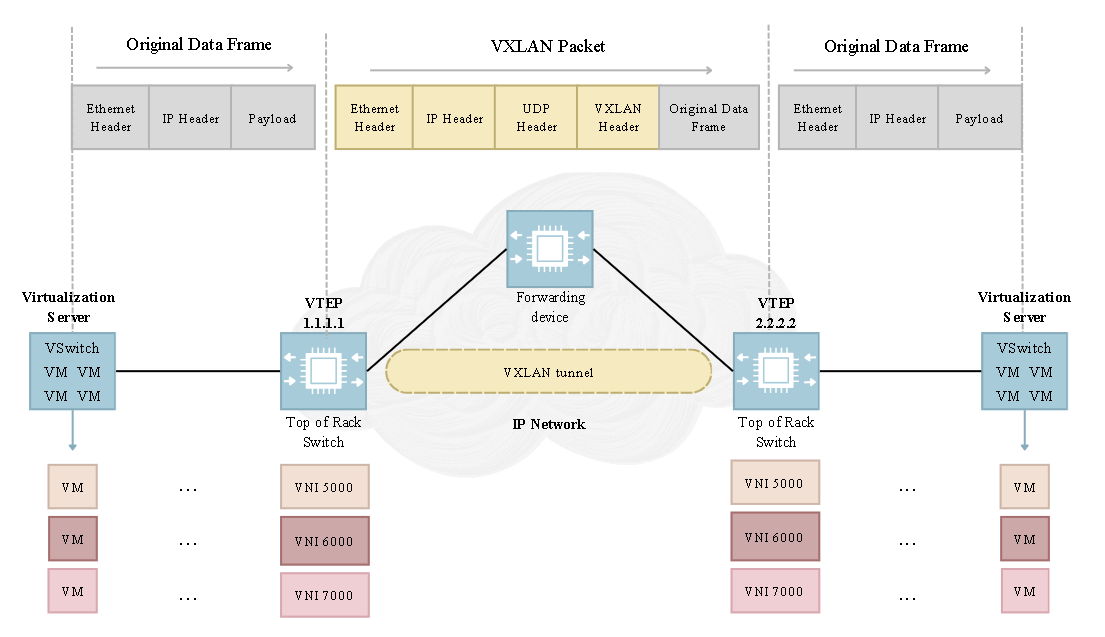
\includegraphics[width=0.9\linewidth]{Figures/VXLANmodel.png}
    \caption{VXLAN network model.}
    \label{VXLANmodel}
\end{figure}

As shown in Figure \ref{VXLANmodel}, VXLAN extends Layer 2 communication over an IP underlay, creating a virtualized network that behaves as a single logical switch interconnecting all endpoints. Any two nodes can communicate transparently through VXLAN tunnels, regardless of the underlying physical topology. From the server's perspective, VXLAN virtualizes the entire infrastructure network into a large "Layer 2 virtual switch", interconnecting all servers as if they resided on the same Layer 2 segment. VXLAN therefore plays an important role in modern data centers as it leads to a significant increase in the number of tenants that the network can effectively isolate and manage. 

In terms of scalability, VXLAN uses a 24-bit VXLAN Network Identifier (VNI), allowing the identification of up to 16 million tenants, far higher than the supported by VLANs. Furthermore, in terms of migration flexibility, VXLAN establishes virtual tunnels between switches across the underlying IP network, effectively virtualizing the infrastructure into a large logical Layer 2 domain that supports large-scale dynamic VM migration.

\subsubsection{VXLAN Encapsulation Structure}

The VXLAN encapsulation process is illustrated in Figure \ref{VXLANpacket}, where the original Ethernet frame is encapsulated within UDP and IPv4 headers and transmitted over the underlay network.

\begin{figure} [H]
    \centering
    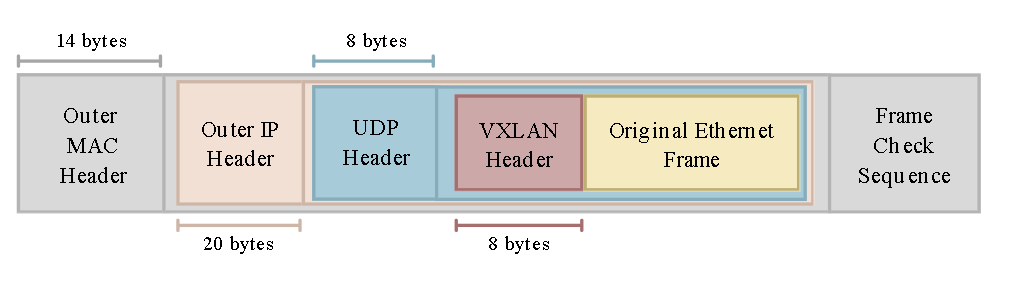
\includegraphics[width=0.65\linewidth]{Figures/VXLANpacket.png}
    \caption{VXLAN packet format. \cite{QSFPtekVXLAN}}
    \label{VXLANpacket}
\end{figure}

The VXLAN header, with a total length of 8 bytes, carries a 24-bit VNI, which uniquely identifies each virtual network or tenants within the VXLAN network. It also contains an 8-bit Flags field, typically set to 00001000, indicating the presence of a valid VNI, along with two reserved fields of 24 and 8 bits that are maintained for future use and protocol consistency.

The VXLAN header and the original Ethernet frame are transported as UDP data. Within the UDP header, the destination port number is fixed at 4789, while the source port number is dynamically calculated using a hash algorithm based on the original Ethernet frame. 

In the outer IP header, the source IP address corresponds to the VXLAN Tunnel Endpoint (VTEP) connected to the source VM, while the destination IP address identifies the VTEP connected to the destination VM. These addresses enable communication across the IP underlay network.

Finally, the outer MAC header, also known as the outer Ethernet header, contains the source and destination MAC addresses used for physical network forwarding. The source MAC address represents the VTEP initiating the transmission, while the destination MAC address corresponds to the next hop on the path toward the destination VTEP.

\subsection{Network Virtualization using Generic Routing Encapsulation}

Network Virtualization using Generic Routing Encapsulation (NVGRE) is a network virtualization mechanism that extends Layer 2 domains over Layer 3 IP infrastructures. Its purpose is to preserve transparency for virtual machines by encapsulating Ethernet frames within IP packets using Generic Routing Encapsulation (GRE), a generic Layer 3 tunnelling protocol. Unlike VXLAN, which employs a MAC-in-UDP encapsulation scheme, NVGRE utilizes MAC-in-IP encapsulation. In addition, while VXLAN uses a 24-bit VXLAN VNI, NVGRE introduces the Virtual Subnet Identifier (VSID), which is carried in the GRE Key field.

The encapsulation structure is illustrated in Figure \ref{nvgre} and operates as follows. When a virtual machine transmits a frame, the source NVGRE endpoint encapsulates the inner Ethernet and IP headers, which form the inner frame. It then adds a GRE header, followed by an outer IP header and an outer Ethernet header, which are used for routing and transmission across the underlay network. The outer Ethernet header constitutes the frame that is physically transmitted across the underlay network. It carries the destination MAC address of the next Layer 2 hop and the source MAC address of the transmitting NVGRE endpoint. Following this, the outer IP header is added at the NVGRE endpoint, containing the source and destination IP addresses that the underlay routers use for packet forwarding.

\begin{figure} [H]
    \centering
    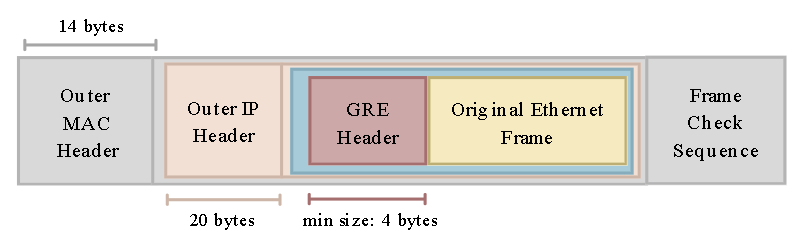
\includegraphics[width=0.6\linewidth]{Figures/NVGREpacket.png}
    \caption{NVGRE packet format. \cite{NVGRE}}
    \label{nvgre}
\end{figure}

The GRE header comprises the VSID field, which is 24 bits in length and enables the identification of up to approximately 16 million virtual networks. It also includes the FlowID field, which increases hash entropy for improved load distribution across equal-cost paths. Following this, the encapsulated tenant traffic, corresponding to the overlay network, includes the inner Ethernet header, containing the MAC addresses of the communicating virtual machines within the virtual network.

From a practical standpoint, this encapsulation process adds several bytes to the frame size. Consequently, the MTU of the underlay network must be increased to prevent fragmentation of the outer packets. Since NVGRE operates over an IP-based underlay, it benefits from Equal-Cost Multi-Path (ECMP) routing, enabling efficient distribution of flows across multiple available paths. The GRE Key field is one of the input parameters in the load-balancing hash calculation used for load balancing across these paths.

In terms of development, NVGRE has been primarily used in Microsoft-based environments, as it originated within Microsoft’s ecosystem and was standardized as the encapsulation method for Hyper-V Network Virtualization (HNV).

\subsection{Geneve}
Geneve is a network encapsulation protocol operating over UDP/IP, designed to provide extensibility through Type-Length-Value (TLV) options. Unlike VXLAN, Geneve decouples a minimal base header from an optional set of extension fields. The packet structure (Figure \ref{geneve}) is composed of outer Ethernet, IP and UDP headers, followed by the Geneve header and the encapsulated payload, which may include Ethernet and IP headers from the original frame.

\begin{figure} [H]
    \centering
    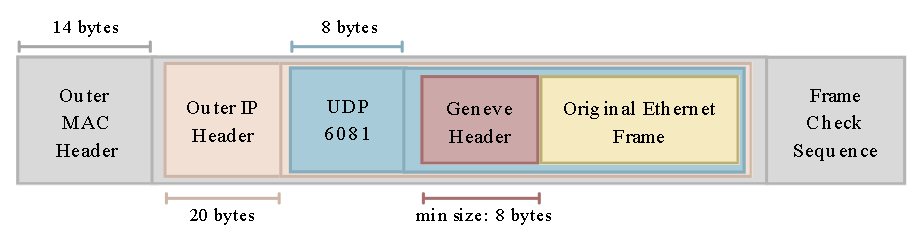
\includegraphics[width=0.65\linewidth]{Figures/genevePacket.png}
    \caption{Geneve packet structure. \cite{Geneve}}
    \label{geneve}
\end{figure}

Analysed from the outside in, we first encounter the Ethernet underlay header, which carriers frames between the GTEP, analogous to the VTEP in VXLAN, and the next hop. This header contains the source MAC of the GTEP and the destination MAC of the Layer 2 next hop. In the next layer, we encounter the IP underlay header, which transports the tunnel between the source and destination GTEPs, using their IP addresses.

Proceeding deeper into the encapsulation, we encounter the UDP header, which Geneve employs to introduce entropy for load balancing. The destination port assigned by IANA is 6081, while the source port is dynamically selected by the GTEP. The final header within the underlay is the Geneve, which is divided into an 8-byte base header and an optional block of Type-Length-Value (TLV) extensions. The base header is composed of several fields, most notably the VNI, which, as with other technologies, is the virtual network identifier. The optional TLV fields are used to attach supplementary information such as telemetry data or operational metadata.

After examining the outer encapsulation, attention shifts to the inner structure of the packet. Immediately following the Geneve header, the payload comprises the overlay frame, representing the original data frame generated by the VM. This frame includes its own set of link-layer, network-layer, and transport-layer headers, corresponding to the standard protocol stack within the virtualized environment.

Geneve is independent of the control plane, and to ensure proper distribution in ECMP, the endpoint varies the source UDP port to increase the entropy of the ECMP hash. Regarding security and Operations, Administration and Maintenance (OAM), the specification defines dedicated fields and behavioural guidelines, including the OAM bit and the handling of critical options, and recommends the use of IPsec when data integrity and confidentiality are required, as the encapsulation mechanism itself does not inherently provide these properties. 

In terms of support, Geneve has been widely adopted in software-based network infrastructures. The Linux kernel integrates a Geneve module that can be configured without relying Open vSwitch (OVS), while VMware NSX-T employs Geneve as its primary transport encapsulation protocol.

\subsection{Stateless Transport Tunnelling}

